\documentclass[11pt]{article}
\usepackage{amsmath}
\usepackage{tikz}
\usepackage[utf8]{inputenc}
\usepackage[T1]{fontenc}
\usepackage{amssymb}
\usepackage{amsmath}

\begin{document}

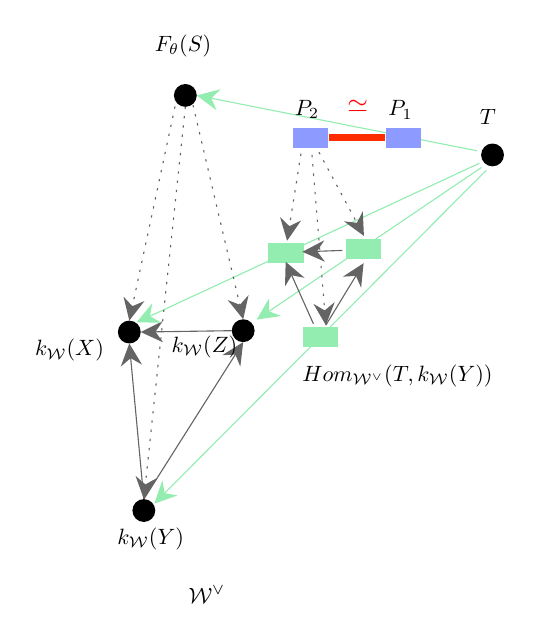
\begin{tikzpicture}[x=0.75pt,y=0.75pt,yscale=-1,xscale=1]

\draw  [draw opacity=0][fill={rgb, 255:red, 0; green, 0; blue, 0 }  ,fill opacity=1 ] (161,158.25) .. controls (161,155.21) and (163.46,152.75) .. (166.5,152.75) .. controls (169.54,152.75) and (172,155.21) .. (172,158.25) .. controls (172,161.29) and (169.54,163.75) .. (166.5,163.75) .. controls (163.46,163.75) and (161,161.29) .. (161,158.25) -- cycle ;
\draw  [draw opacity=0][fill={rgb, 255:red, 0; green, 0; blue, 0 }  ,fill opacity=1 ] (215.87,157.6) .. controls (215.87,154.56) and (218.33,152.1) .. (221.37,152.1) .. controls (224.4,152.1) and (226.87,154.56) .. (226.87,157.6) .. controls (226.87,160.64) and (224.4,163.1) .. (221.37,163.1) .. controls (218.33,163.1) and (215.87,160.64) .. (215.87,157.6) -- cycle ;
\draw  [draw opacity=0][fill={rgb, 255:red, 0; green, 0; blue, 0 }  ,fill opacity=1 ] (168,244.25) .. controls (168,241.21) and (170.46,238.75) .. (173.5,238.75) .. controls (176.54,238.75) and (179,241.21) .. (179,244.25) .. controls (179,247.29) and (176.54,249.75) .. (173.5,249.75) .. controls (170.46,249.75) and (168,247.29) .. (168,244.25) -- cycle ;
\draw [color={rgb, 255:red, 100; green, 100; blue, 100 }  ,draw opacity=1 ]   (173.5,238.75) -- (219.76,165.64) ;
\draw [shift={(221.37,163.1)}, rotate = 122.32] [fill={rgb, 255:red, 100; green, 100; blue, 100 }  ,fill opacity=1 ][line width=0.08]  [draw opacity=0] (10.72,-5.15) -- (0,0) -- (10.72,5.15) -- (7.12,0) -- cycle    ;
\draw [color={rgb, 255:red, 100; green, 100; blue, 100 }  ,draw opacity=1 ]   (173.5,238.75) -- (166.78,166.74) ;
\draw [shift={(166.5,163.75)}, rotate = 84.67] [fill={rgb, 255:red, 100; green, 100; blue, 100 }  ,fill opacity=1 ][line width=0.08]  [draw opacity=0] (10.72,-5.15) -- (0,0) -- (10.72,5.15) -- (7.12,0) -- cycle    ;
\draw [color={rgb, 255:red, 100; green, 100; blue, 100 }  ,draw opacity=1 ]   (215.87,157.6) -- (175,158.21) ;
\draw [shift={(172,158.25)}, rotate = 359.15] [fill={rgb, 255:red, 100; green, 100; blue, 100 }  ,fill opacity=1 ][line width=0.08]  [draw opacity=0] (10.72,-5.15) -- (0,0) -- (10.72,5.15) -- (7.12,0) -- cycle    ;
\draw  [draw opacity=0][fill={rgb, 255:red, 0; green, 0; blue, 0 }  ,fill opacity=1 ] (188,44.25) .. controls (188,41.21) and (190.46,38.75) .. (193.5,38.75) .. controls (196.54,38.75) and (199,41.21) .. (199,44.25) .. controls (199,47.29) and (196.54,49.75) .. (193.5,49.75) .. controls (190.46,49.75) and (188,47.29) .. (188,44.25) -- cycle ;
\draw  [draw opacity=0][fill={rgb, 255:red, 0; green, 0; blue, 0 }  ,fill opacity=1 ] (336,72.92) .. controls (336,69.88) and (338.46,67.42) .. (341.5,67.42) .. controls (344.54,67.42) and (347,69.88) .. (347,72.92) .. controls (347,75.95) and (344.54,78.42) .. (341.5,78.42) .. controls (338.46,78.42) and (336,75.95) .. (336,72.92) -- cycle ;
\draw [color={rgb, 255:red, 147; green, 237; blue, 177 }  ,draw opacity=1 ][fill={rgb, 255:red, 147; green, 237; blue, 177 }  ,fill opacity=1 ]   (335.2,76.93) -- (172.72,152.32) ;
\draw [shift={(170,153.58)}, rotate = 335.11] [fill={rgb, 255:red, 147; green, 237; blue, 177 }  ,fill opacity=1 ][line width=0.08]  [draw opacity=0] (10.72,-5.15) -- (0,0) -- (10.72,5.15) -- (7.12,0) -- cycle    ;
\draw [color={rgb, 255:red, 147; green, 237; blue, 177 }  ,draw opacity=1 ][fill={rgb, 255:red, 147; green, 237; blue, 177 }  ,fill opacity=1 ]   (338.53,80.27) -- (180.65,238.81) ;
\draw [shift={(178.53,240.93)}, rotate = 314.88] [fill={rgb, 255:red, 147; green, 237; blue, 177 }  ,fill opacity=1 ][line width=0.08]  [draw opacity=0] (10.72,-5.15) -- (0,0) -- (10.72,5.15) -- (7.12,0) -- cycle    ;
\draw [color={rgb, 255:red, 147; green, 237; blue, 177 }  ,draw opacity=1 ][fill={rgb, 255:red, 147; green, 237; blue, 177 }  ,fill opacity=1 ]   (336.2,78.93) -- (230.35,150.58) ;
\draw [shift={(227.87,152.27)}, rotate = 325.91] [fill={rgb, 255:red, 147; green, 237; blue, 177 }  ,fill opacity=1 ][line width=0.08]  [draw opacity=0] (10.72,-5.15) -- (0,0) -- (10.72,5.15) -- (7.12,0) -- cycle    ;
\draw  [draw opacity=0][fill={rgb, 255:red, 147; green, 237; blue, 177 }  ,fill opacity=1 ] (233.55,115.26) -- (250.48,115.26) -- (250.48,124.93) -- (233.55,124.93) -- cycle ;
\draw  [draw opacity=0][fill={rgb, 255:red, 147; green, 237; blue, 177 }  ,fill opacity=1 ] (270.88,113.26) -- (287.81,113.26) -- (287.81,122.93) -- (270.88,122.93) -- cycle ;
\draw  [draw opacity=0][fill={rgb, 255:red, 147; green, 237; blue, 177 }  ,fill opacity=1 ] (250.07,155.76) -- (267,155.76) -- (267,165.44) -- (250.07,165.44) -- cycle ;
\draw [color={rgb, 255:red, 100; green, 100; blue, 100 }  ,draw opacity=1 ]   (255.2,154.27) -- (243.06,127.15) ;
\draw [shift={(241.83,124.42)}, rotate = 65.88] [fill={rgb, 255:red, 100; green, 100; blue, 100 }  ,fill opacity=1 ][line width=0.08]  [draw opacity=0] (10.72,-5.15) -- (0,0) -- (10.72,5.15) -- (7.12,0) -- cycle    ;
\draw [color={rgb, 255:red, 100; green, 100; blue, 100 }  ,draw opacity=1 ]   (261.2,154.93) -- (277.81,127.66) ;
\draw [shift={(279.37,125.1)}, rotate = 121.34] [fill={rgb, 255:red, 100; green, 100; blue, 100 }  ,fill opacity=1 ][line width=0.08]  [draw opacity=0] (10.72,-5.15) -- (0,0) -- (10.72,5.15) -- (7.12,0) -- cycle    ;
\draw [color={rgb, 255:red, 100; green, 100; blue, 100 }  ,draw opacity=1 ] [dash pattern={on 0.84pt off 2.51pt}]  (188.53,49.6) -- (167.13,149.82) ;
\draw [shift={(166.5,152.75)}, rotate = 282.06] [fill={rgb, 255:red, 100; green, 100; blue, 100 }  ,fill opacity=1 ][line width=0.08]  [draw opacity=0] (10.72,-5.15) -- (0,0) -- (10.72,5.15) -- (7.12,0) -- cycle    ;
\draw [color={rgb, 255:red, 100; green, 100; blue, 100 }  ,draw opacity=1 ] [dash pattern={on 0.84pt off 2.51pt}]  (197.2,48.93) -- (220.68,149.18) ;
\draw [shift={(221.37,152.1)}, rotate = 256.82] [fill={rgb, 255:red, 100; green, 100; blue, 100 }  ,fill opacity=1 ][line width=0.08]  [draw opacity=0] (10.72,-5.15) -- (0,0) -- (10.72,5.15) -- (7.12,0) -- cycle    ;
\draw [color={rgb, 255:red, 100; green, 100; blue, 100 }  ,draw opacity=1 ] [dash pattern={on 0.84pt off 2.51pt}]  (193.5,49.75) -- (173.82,235.77) ;
\draw [shift={(173.5,238.75)}, rotate = 276.04] [fill={rgb, 255:red, 100; green, 100; blue, 100 }  ,fill opacity=1 ][line width=0.08]  [draw opacity=0] (10.72,-5.15) -- (0,0) -- (10.72,5.15) -- (7.12,0) -- cycle    ;
\draw [color={rgb, 255:red, 100; green, 100; blue, 100 }  ,draw opacity=1 ]   (269.2,118.93) -- (252.86,119.5) ;
\draw [shift={(249.87,119.6)}, rotate = 358.03] [fill={rgb, 255:red, 100; green, 100; blue, 100 }  ,fill opacity=1 ][line width=0.08]  [draw opacity=0] (10.72,-5.15) -- (0,0) -- (10.72,5.15) -- (7.12,0) -- cycle    ;
\draw [color={rgb, 255:red, 147; green, 237; blue, 177 }  ,draw opacity=1 ]   (334,70.92) -- (201.94,44.83) ;
\draw [shift={(199,44.25)}, rotate = 11.17] [fill={rgb, 255:red, 147; green, 237; blue, 177 }  ,fill opacity=1 ][line width=0.08]  [draw opacity=0] (10.72,-5.15) -- (0,0) -- (10.72,5.15) -- (7.12,0) -- cycle    ;
\draw  [draw opacity=0][fill={rgb, 255:red, 141; green, 154; blue, 255 }  ,fill opacity=1 ] (289.97,59.92) -- (306.9,59.92) -- (306.9,69.6) -- (289.97,69.6) -- cycle ;
\draw  [draw opacity=0][fill={rgb, 255:red, 141; green, 154; blue, 255 }  ,fill opacity=1 ] (245.27,59.84) -- (262.2,59.84) -- (262.2,69.52) -- (245.27,69.52) -- cycle ;
\draw [color={rgb, 255:red, 100; green, 100; blue, 100 }  ,draw opacity=1 ] [dash pattern={on 0.84pt off 2.51pt}]  (249.2,72.27) -- (243,111.3) ;
\draw [shift={(242.53,114.27)}, rotate = 279.02] [fill={rgb, 255:red, 100; green, 100; blue, 100 }  ,fill opacity=1 ][line width=0.08]  [draw opacity=0] (10.72,-5.15) -- (0,0) -- (10.72,5.15) -- (7.12,0) -- cycle    ;
\draw [color={rgb, 255:red, 100; green, 100; blue, 100 }  ,draw opacity=1 ] [dash pattern={on 0.84pt off 2.51pt}]  (254.53,72.93) -- (260.96,151.94) ;
\draw [shift={(261.2,154.93)}, rotate = 265.35] [fill={rgb, 255:red, 100; green, 100; blue, 100 }  ,fill opacity=1 ][line width=0.08]  [draw opacity=0] (10.72,-5.15) -- (0,0) -- (10.72,5.15) -- (7.12,0) -- cycle    ;
\draw [color={rgb, 255:red, 100; green, 100; blue, 100 }  ,draw opacity=1 ] [dash pattern={on 0.84pt off 2.51pt}]  (257.87,71.6) -- (278.11,109.29) ;
\draw [shift={(279.53,111.93)}, rotate = 241.76] [fill={rgb, 255:red, 100; green, 100; blue, 100 }  ,fill opacity=1 ][line width=0.08]  [draw opacity=0] (10.72,-5.15) -- (0,0) -- (10.72,5.15) -- (7.12,0) -- cycle    ;
\draw [color={rgb, 255:red, 255; green, 44; blue, 0 }  ,draw opacity=1 ][fill={rgb, 255:red, 255; green, 44; blue, 0 }  ,fill opacity=1 ][line width=2.25]    (289.87,64.58) -- (262.67,64.58) ;

% Text Node
\draw (194.68,20.5) node  [xscale=0.8,yscale=0.8] [align=left] {\begin{minipage}[lt]{29.72pt}\setlength\topsep{0pt}
	$\displaystyle F_{\theta }( S)$
	\end{minipage}};
% Text Node
\draw (132.33,167) node  [xscale=0.8,yscale=0.8] [align=left] {\begin{minipage}[lt]{21.08pt}\setlength\topsep{0pt}
	$\displaystyle k_{\mathcal{W}}( X)$
	\end{minipage}};
% Text Node
\draw (198.17,165.5) node  [xscale=0.8,yscale=0.8] [align=left] {\begin{minipage}[lt]{21.08pt}\setlength\topsep{0pt}
	$\displaystyle k_{\mathcal{W}}( Z)$
	\end{minipage}};
% Text Node
\draw (172,258) node  [xscale=0.8,yscale=0.8] [align=left] {\begin{minipage}[lt]{21.08pt}\setlength\topsep{0pt}
	$\displaystyle k_{\mathcal{W}}( Y)$
	\end{minipage}};
% Text Node
\draw (203,285) node  [xscale=0.8,yscale=0.8] [align=left] {\begin{minipage}[lt]{14.96pt}\setlength\topsep{0pt}
	$\displaystyle \mathcal{W}^{\lor }$
	\end{minipage}};
% Text Node
\draw (342.02,54.5) node  [xscale=0.8,yscale=0.8] [align=left] {\begin{minipage}[lt]{12.49pt}\setlength\topsep{0pt}
	$\displaystyle T$
	\end{minipage}};
% Text Node
\draw (282.28,49.71) node  [font=\large,xscale=0.8,yscale=0.8] [align=left] {\begin{minipage}[lt]{20.09pt}\setlength\topsep{0pt}
	{\large  \textcolor[rgb]{1,0,0}{{$\simeq $}}}
	\end{minipage}};
% Text Node
\draw (297.96,51.17) node  [xscale=0.8,yscale=0.8] [align=left] {\begin{minipage}[lt]{12.49pt}\setlength\topsep{0pt}
	$\displaystyle P_{1}$
	\end{minipage}};
% Text Node
\draw (299.08,179.35) node  [xscale=0.8,yscale=0.8] [align=left] {\begin{minipage}[lt]{92.31pt}\setlength\topsep{0pt}
	$\displaystyle Hom_{\mathcal{W}^{\lor }}( T,k_{\mathcal{W}}( Y))$
	\end{minipage}};
% Text Node
\draw (252.96,50.92) node  [xscale=0.8,yscale=0.8] [align=left] {\begin{minipage}[lt]{12.49pt}\setlength\topsep{0pt}
	$\displaystyle P_{2}$
	\end{minipage}};


\end{tikzpicture}

\end{document}